\documentclass[11pt,letterpaper,reqno]{article}

\textwidth      =  6in
\textheight     =  8.25in
\oddsidemargin  =  18pt
\evensidemargin =  18pt
\topmargin      =  0.00in

\usepackage[utf8]{inputenc}
\usepackage[spanish]{babel}
\usepackage{amsmath}
\usepackage{amsfonts}
\usepackage{amssymb}
\usepackage{graphicx}
\usepackage{hyperref}
\graphicspath{{img/}}

\title{Análisis de dos Clasificadores}
\author{Abraham Toriz\\ Jesús Mejía\\ Luis Cortés\\ Roberto Saucedo}

\newtheorem{definition}{Definición}[section]

\begin{document}
\pagestyle{empty}
\begin{minipage}{.15\textwidth}
	
\includegraphics[scale=.22]{uv.eps}
\end{minipage}
\begin{minipage}{.7\textwidth}
\centering
{\huge \sc Universidad Veracruzana}\\
{\LARGE \sc Facultad de Matemáticas}
\end{minipage}
\begin{minipage}{.15\textwidth}
	\begin{flushright}
		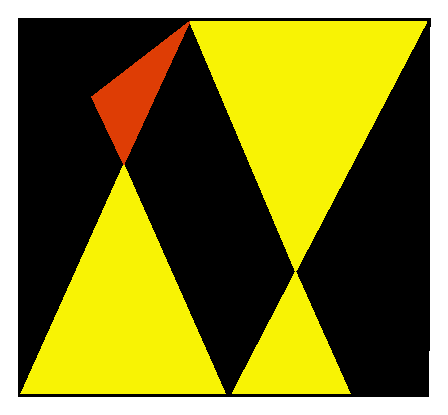
\includegraphics[scale=.22]{matematicas.eps}
	\end{flushright}
\end{minipage}

\vspace{.7cm}
\begin{center}
{\huge \bf
	Análisis de dos Clasificadores
}
\\[1.5cm]
{ \Huge
	T A R E A
}
\\[1.5cm]

{ \large
	Que para pasar la materia
}
\\[.5cm]
{ \LARGE \bf
	Temas Selectos de Estadística
}
\\[1cm]
Presentan los siguientes\\[1cm]
{ \Large
I N T E G R A N T E S:
}\\
{ \LARGE \bf
	Abraham Toriz\\
	Jesús Mejía\\
	Luis Cortés\\
	Roberto Saucedo
}\\[1cm]
{ \Large
CATEDRÁTICO:
}\\
{ \LARGE \bf
	Martha Lorena Avendaño
}
\end{center}
\vspace{1.5cm}
\begin{minipage}{.5\textwidth}
\centering
Xalapa, Veracruz
\end{minipage}
\begin{minipage}{.5\textwidth}
\centering
4 de septiembre de 2015
\end{minipage}

%-----------------%
\pagebreak
\pagestyle{plain}

\begin{abstract}
En el afán del ser humano por reducir el esfuerzo para concretar una tarea se han desarrollado técnicas y conocimientos que suplen a la intuicíón. Una de estas tareas es la clasificación de objetos para tomar mejores decisiones. Con tal fin en la matemática, por medio de la estadística, se tienen métodos que permiten aproximar un modelo de clasificación de datos basados en una muestra. En este proyecto estudiamos dos de ellos: el modelo de regresión logística y el modelo de los $n$ vecinos más cercanos.
\end{abstract}

\section{Consideraciones}

La elección de la notación para los escritos científicos siempre es una tarea difícil, así que adoptaremos el mismo que los convencionalismos de la ESL (vea \cite{sLearning2013}). Usaremos $N$ para representar el número de datos distintos u observaciones en nuestras muestras y $p$ denotará el número de variables que están disponibles para hacer predicciones.\\

Para poder clasificar los datos por medio de un algoritmo es necesario hacer \textit{suposiciones}. Una de las suposiciones necesarias es pensar que existe algún modelo $f$ (aunque no lo conozcamos) que nos proporciona la clasificación de los datos

$$
Y = f(X) + \varepsilon,
$$

donde $X$ es el dato a clasificar, $Y$ la clase a la que pertenece y $\epsilon$  una variable aleatoria independiente de $X$ con media cero que se relaciona con el error introducido por el medio.

Con esta información tratamos de construir una estimación del modelo $f$ que llamamos $\hat{f}$ con la cual tratamos de aproximar $Y$. A esta aproximación la denotamos por $\hat{Y}$.

$$
\hat{Y} = \hat{f}(X)
$$

\subsection{Tipos de modelos}

Trabajaremos con dos tipos de modelos según la forma en que estos se construyen a partir de los supuestos.

\begin{itemize}
	\item \textbf{Modelos paramétricos} Son aquellos que dependen de parámetros y estos parámetros se estiman bajo algún criterio del \textit{mejor ajuste} a partir de los datos muestra. Se espera que estos datos sean suficientemente buenos (y los parámetros bien escogidos) para que el modelo clasifique bien.
	\item \textbf{Modelos no paramétricos} No dependen de parámetros sin embargo se ajusta el clasificador a partir de una muestra representativa de los datos a clasificar.
\end{itemize}

\section{Regresión Logística}

Supongamos que tenemos $N$ observaciones (con clases $Y=1$ o $Y=2$). En cierto momento nos encontramos un nuevo dato $X$ del cual no se conoce la clase que pertenece. Ahora nuestro trabajo es encontrar la función $p$ de probabilidad que nos indique la clase de $X$ en función de las $N$ observaciones previas. ¿Cómo podríamos modelar la relación ente $p(X) = P(Y=1|X)$ y $X$? Pues bien, sabemos que podemos utilizar un modelo de regresión lineal para representar dichas probabilidades:
\begin{equation*}
p(X) = \beta_0 + \beta_1X.
\end{equation*}

Sin embargo nos gustaría una función $P$ tal que modele la probabilidad (i.e. $\forall X$, $P(X)\in[0,\; 1]$). En la regresión logística, se usa la función \textit{logística},

\begin{equation}
	\label{eqn:func_logistica}
	P(X) = \frac{e^{\beta_0 + \beta_1^{T} X}}{1+e^{\beta_0 + \beta_1^{T}X}},
\end{equation}
donde:
\begin{itemize}
	\item[$\beta_0$]$\in \mathbb{R}$
	\item[$\beta_1^T$] es un vector con $p$ entradas.
\end{itemize}
Para ajustar el modelo (\ref{eqn:func_logistica}), usamos el método de la máxima verosimilitud. Esta técnica propone una función paramétrica para la clasificación binaria:
\begin{equation}
	\label{eqn:func_L}
	\mathcal{L}(\beta_{0}, \beta_{1}) = \prod_{i=1}^{N}p(X_i)^{Y_i}[1-p(X_{i})]^{1-Y_i}
\end{equation}
Los estimadores $\hat{\beta_0}$ y $\hat{\beta_1}$ se eligen de tal que manera que maximicen la función $\mathcal{L}$ (conocida como función de verosimilitud). Las máxima verosimilitud es una aproximación general que se usa para ajustar modelos lineales y no lineales.\\

Si sustituimos la ecuación (\ref{eqn:func_logistica}) en (\ref{eqn:func_L}) y desarrollando obtenemos,
$$
\mathcal{L}(\beta_{0}, \beta_{1}) =  \prod_{i=1}^{N} \left[ \frac{e^{\beta_0 + \beta_1^{T} X}}{1+e^{\beta_0 + \beta_1^{T}X}} \right]^{Y_i} \left[\frac{1}{1+e^{\beta_0 + \beta_1^{T}X}} \right]^{1-Y_i}.
$$
La función anterior es difícil de trabajar, puesto que está dado por un producto y es más difícil tratarla que si se tratara de una suma. Así, apliquemos el logaritmo para obtener:
$$
\ell(\beta_{0}, \beta_{1}) = \log\mathcal{L}(\beta_{0}, \beta_{1}) = \sum_{i=1}^{N}\left[ Y_i\left[ \frac{e^{\beta_0 + \beta_1^{T} X}}{1+e^{\beta_0 + \beta_1^{T}X}} \right] +  (1-Y_i)\left[\frac{1}{1+e^{\beta_0 + \beta_1^{T}X}} \right] \right].
$$

Ahora, solo resta maximizar dicha función, a través métodos numéricos apropiados. 

\section{Los $k$ Vecinos más Cercanos}

La idea básica sobre la que se fundamenta este clasificador es que una nueva muestra será clasificada a la clase más frecuente a la que pertenecen sus vecinos más cercanos ($k$-nn por sus siglas en inglés).\\

$k$-nn es un algoritmo perezoso, esto es, que durante el entrenamiento, solo guarda instancias y no construye ningún modelo, tampoco hace supuestos sobre la distribución que siguen los datos, por lo tanto es no paramétrico.\\

Dado un conjunto de datos $ X= \left\lbrace X_1,\;X_2, \ldots ,\; X_p \right\rbrace $ y un conjunto de clases $ C= \left\lbrace C_1,\;C_2, \ldots ,\; C_m \right\rbrace $, el  problema de clasificación es encontrar una función $ f:X \longrightarrow C $ tal que cada $ X_i $ es asignada a una clase $ C_j $.\\

La fase de entrenamiento del algoritmo consiste en almacenar los vectores característicos y las etiquetas de las clases de los ejemplos de entrenamiento.  En la fase de clasificación, la evaluación del ejemplo (del que no se conoce su clase) es representada por un vector en el espacio característico.
$ x = \left\lbrace x_1,x_2, ... , x_m \right\rbrace $
Se calcula la distancia entre los vectores almacenados y el nuevo vector, generalmente se usa la distancia euclidiana

$$
d(x_i,x_j)=\sqrt{\sum_{r=1}^{p} (x_{ri}-x_{rj})^2} 
$$

y se seleccionan los $ k $ ejemplos más cercanos.\\

El nuevo ejemplo es clasificado con la clase que más se repite en los vectores seleccionados. Este método supone que los vecinos más cercanos nos dan la mejor clasificación y esto se hace utilizando todos los atributos. Los valores de los atributos del i-esimo ejemplo con $ i \in \left\lbrace 1, \ldots , n \right\rbrace $ se representan por el vector p-dimensional.\\

El problema de dicha suposición es que es posible que se tengan muchos atributos irrelevantes que dominen sobre la clasificación: dos atributos relevantes perderían peso entre otros veinte irrelevantes.\\

Para corregir el posible sesgo se puede asignar un peso a las distancias de cada atributo, dándole así mayor importancia a los atributos más relevantes. Otra posibilidad consiste en tratar de determinar o ajustar los pesos con ejemplos conocidos de entrenamiento. Finalmente, antes de asignar pesos es recomendable identificar y eliminar los atributos que se consideran irrelevantes.\\

La mejor elección de $ k $ depende fundamentalmente de los datos; generalmente, valores grandes de $ k $ reducen el efecto de ruido en la clasificación, pero crean límites entre clases parecidas. Un buen $ k $ puede ser seleccionado mediante una optimización de uso.\\

La exactitud de este algoritmo puede ser severamente degradada por la presencia de ruido o características irrelevantes, o si las escalas de características no son consistentes con lo que uno considera importante.

\section{Análisis de datos}

A continuación se presenta una comparativa de la aplicación de estos dos modelos previamente mencionados.

En el primer caso (fig. \ref{fig:fig01}) se estudian dos conjuntos con medias distintas y poca varianza, donde es difícil que un punto de un conjunto se encuentre cerca del otro conjunto.

\begin{figure}[h]
	\begin{center}
		\includegraphics[scale=.4]{fig01}
	\end{center}
	\caption{Conjuntos \textit{ajenos}, 99\% de éxito en ambos clasificadores.}
	\label{fig:fig01}
\end{figure}

En este caso tanto el clasificador $k$-nn como la regresión logística obtuvieron un resultado satisfactorio clasificando adecuadamente el 99\% de la muestra. Sin embargo conforme los conjuntos van acercando sus medias este resultado empieza a ser menos preciso como se puede observar en la figura \ref{fig:fig02}

\begin{figure}[h]
	\begin{center}
		\includegraphics[scale=0.4]{fig02}
	\end{center}
	\caption{Conforme los conjuntos acercan sus medias la precisión disminuye en ambos casos: 93\% para la regresión logística y 88\% para $k$-nn.}
	\label{fig:fig02}
\end{figure}

Si se presenta el caso de que los conjuntos compartan la media y la varianza, su clasificación se vuelve casi imposible, siendo mejor lanzar una moneda y decidir el resultado que fiarse de algún método (figure \ref{fig:fig03})

\begin{figure}[h]
	\begin{center}
		\includegraphics[scale=0.4]{fig03}
	\end{center}
	\caption{La media y la varianza son iguales, no es posible distinguir con certeza los conjuntos entre sí usando estos clasificadores, los resultados de la evaluación son 54\% de éxito para la regresión, 48\% para $k$-nn}
	\label{fig:fig03}
\end{figure}

Ahora, si suponemos dos conjuntos con medias distintas y mucha varianza observaremos que se comenzarán a mezclar, al mezclarse habrá una región donde podremos encontrar elementos de ambas clases y al preguntar los los vecinos más cercanos puede suceder que se encuentren más de una u otra clase. En este experimento la regresión logística obtuvo un mejor desempeño como se observa en la figura \ref{fig:fig04}

\begin{figure}[h]
	\begin{center}
		%\includegraphics[scale=0.4]{fig04}
	\end{center}
	\caption{Cuando los conjuntos se mezclan, $k$-nn puede confundirse (87\% de éxito), pareciera que la regresión logísitca es una mejor opción con el 92\% de éxito}
	\label{fig:fig04}
\end{figure}

Sin embargo, en dos experimentos más se observó un comportamiento diferente. En el primero se plantean dos conjuntos con medias iguales pero varianzas desalineadas en los ejes, de forma que existe una región de puntos mixta en el centro y cuatro regiones más o menos bien definidas en cuanto a clase (figura \ref{fig:fig05}). En el segundo se observa un cluster de elementos de la clase 1 de poca varianza sumergido en una región de elementos de la clase 2 de mayor varianza (figura \ref{fig:fig06}). En ambos casos $k$-nn demostró tener un mejor desempeño para clasificar los datos.

\begin{figure}[h]
	\begin{center}
		\includegraphics[scale=0.4]{fig05}
	\end{center}
	\caption{Diseño en \textit{cruz} de dos conjuntos. El clasificador de la regresión logística tiene un muy pobre desempeño (49\%) mientras que $k$-nn se mantiene aceptable con 70\% de aciertos}
	\label{fig:fig05}
\end{figure}

\begin{figure}[h]
	\begin{center}
		\includegraphics[scale=0.4]{fig06}
	\end{center}
	\caption{Cluster. También en este caso $k$-nn logra un mejor resultado quizá debido a la cercanía de los puntos de una de las clases. Obtiene 72\% de aciertos mientras que la regresión logística apenas supera el tiro de la moneda con 51\%}
	\label{fig:fig06}
\end{figure}

\section{Conclusiones}

Pese a la formalidad con que se construye la teoría alrededor del clasificador de la regresión logística (o quizá debido a ella) este supone mayores dificultades al momento de la implementación para obtener mejores resultados. Por su parte el clasificador $k$-nn ofrece un prncipio sencillo y funcional para clasificar los datos.\\

Sin duda la idea de optimizar para un conjunto de parámetros puede mejorarse por ejemplo encontrando cotas para estos mismos, quizá esto y algunas otras técnicas proporcionen un mejor acercamiento al resultado esperado.\\

En esta sección se desarrollarán algunos experimentos en lo que pondremos a prueba los modelos poniendo a prueba la efectividad de éstos. \cite{gitEnlace}

\clearpage

\bibliographystyle{plain}
\bibliography{referencias}

\end{document}
